% ============================================================
% 软件功能与交互界面规划 — 领导版（一张图看懂买了什么、看到什么）
% 口径对齐: 报价表 V10（5 板块 48 计价项）/ 全景论证 / 附件②③④⑥ / dgiot_lite 底座
% 编译: xelatex -interaction=nonstopmode 规划-软件功能与交互界面.tex
% ============================================================
\documentclass[11pt,a4paper]{ctexart}
\usepackage{xeCJK}
\usepackage{graphicx}
\usepackage{float}
\usepackage{fancyhdr}
\usepackage{hyperref}
\usepackage{geometry}
\usepackage{booktabs}
\usepackage{enumitem}
\usepackage{array}
\usepackage{xcolor}
\usepackage{longtable}
\usepackage{tikz}
\usetikzlibrary{arrows.meta, positioning, calc}
\definecolor{l1}{HTML}{00b4d8}
\definecolor{l2}{HTML}{10b981}
\definecolor{l3}{HTML}{f59e0b}
\definecolor{accent}{HTML}{00b4d8}

% 字体
\setCJKmainfont{Microsoft YaHei}
% 带圈数字 ①-⑳ 划入 CJK 字符类（否则 Latin 字体缺字）
\xeCJKDeclareCharClass{CJK}{"2460 -> "2473}

% 页面
\geometry{a4paper, margin=2.2cm}

% 节标题压缩
\ctexset{section={beforeskip=10pt, afterskip=6pt}}

% 页眉页脚
\pagestyle{fancy}
\fancyhead[L]{时序数据采集与应用管理系统 — 软件功能与交互界面规划}
\fancyhead[R]{领导版}
\fancyfoot[C]{\thepage}

\hypersetup{
  colorlinks=true, linkcolor=black, urlcolor=blue,
  pdftitle={软件功能与交互界面规划——时序数据采集与应用管理系统},
}

\begin{document}

\begin{center}
{\Huge\bfseries 软件功能与交互界面规划}\\[6pt]
{\large 时序数据采集与应用管理系统 —— 一张图看懂：买了什么功能、打开系统看到什么}\\[6pt]
{\small 配套：新架构图-数据流图 + 报价书 + 报价表 V10（5 板块 48 计价项）\quad 2026-08}
\end{center}

\vspace{0.5em}
\noindent\hrulefill
\vspace{0.5em}

% ═══════════════════════════════════════════
\section{功能全景一张图}

本系统软件按\textbf{五层功能架构}组织，从底层采集到顶层展示环环贯通；每一层都能在报价表中找到对应的开发项，\textbf{报价不是"买一堆零件"，而是一条完整的数据流水线}：

\begin{figure}[H]\centering
\begin{tikzpicture}[
  font=\small,
  layer/.style={draw, rounded corners=3pt, align=center, inner sep=6pt, text width=14.0cm},
  lab/.style={font=\footnotesize\bfseries, fill=white, inner sep=2pt},
  arrow/.style={-{Stealth}, very thick, black!70}
]
% 五层（positioning 自动堆叠，防重叠）
\node[layer, fill=orange!10] (L1) {
  {\large\bfseries ⑤ 应用展示层 —— 领导与运维每天看到的}\\[3pt]
  数据驾驶舱（大屏）· 设备管理 · 设备接入 · 算法管理 · 告警中心 · 数据服务 · 可视化 · 系统管理\\[2pt]
  {\footnotesize 对应：边缘中枢平台开发（板块一）}
};
\node[layer, fill=blue!8, below=1.6cm of L1] (L2) {
  {\large\bfseries ④ 计算分析层 —— 数据在入库前就被算好}\\[3pt]
  定制化流式计算引擎（15 种内置算法 + 每作业区定制注册）· 流式告警规则引擎 · 可视化规则编排\\[2pt]
  {\footnotesize 对应：定制化流式计算引擎 + 告警规则引擎 + 作业区定制（板块一、板块四-【B】【C】）}
};
\node[layer, fill=green!8, below=1.6cm of L2] (L3) {
  {\large\bfseries ③ 存储与消息层 —— 数据存得住、传得动}\\[3pt]
  混合存储引擎（时序库 + 关系库，主数据唯一源头）· 数据生命周期管理 · 边缘分级存储\\[2pt]
  消息中间件与边云同步（边缘 $\rightarrow$ DMZ $\rightarrow$ 中心全链路贯通）\\[2pt]
  {\footnotesize 对应：混合存储引擎 + 消息中间件 + 边缘中枢（板块一、板块二）}
};
\node[layer, fill=gray!10, below=1.6cm of L3] (L4) {
  {\large\bfseries ② 采集接入层 —— 全终端、全协议、双路采集}\\[3pt]
  多协议解析引擎（A11 专有协议 + 10 余种工业协议）· 双路采集（静态 IP 客户端主动采集 / 动态 IP 抢占原地址端口桥接转发）\\[2pt]
  设备统一动态感知（静态 IP + 移动网关）· 10 家网关厂家适配 · 智能动态调频 · 断网缓存补传\\[2pt]
  {\footnotesize 对应：多协议解析引擎 + 边缘采集模块 + 采集策略多样化定制（板块一、板块三、板块四-【A】）}
};
\node[layer, fill=gray!25, below=1.6cm of L4] (L5) {
  {\large\bfseries ① 终端设备层 —— 利旧，不改不动}\\[3pt]
  静态 IP 终端（有线/固定链路，设备侧服务端）· 动态 IP 终端（4G 移动网关，设备侧客户端）\\[2pt]
  {\footnotesize A11 系统保留运行，全部既有设备与配置原样不动（前约束）}
};

% 数据流主线（图内底部提示）
\node[lab, below=0.25cm of L5, text width=14cm, align=center] {数据流主线：采集 $\rightarrow$ 计算 $\rightarrow$ 存储 $\rightarrow$ 展示};
\end{tikzpicture}
\caption{五层功能架构——从终端到领导屏幕的数据流水线，每层对应报价开发项}
\end{figure}

\begin{center}
\large\bfseries 领导一句话：\underline{底层设备全部利旧、一条数据流水线贯通，顶层一张大屏看清全油田}
\end{center}

% ═══════════════════════════════════════════
\section{技术服务内容：七个一级模块}

系统技术服务内容划分为\textbf{七个一级模块}，每个模块采用"总—分"结构组织：先简要说明模块定位，再展开具体服务内容。

\begin{table}[H]\centering
\caption{七模块总览（模块 $\rightarrow$ 核心服务 $\rightarrow$ 平台价值）}
\begin{tabular}{p{2.2cm} p{3.8cm} p{7.5cm}}
\toprule
\textbf{一级模块} & \textbf{核心服务} & \textbf{平台价值} \\
\midrule
\textbf{1. 多维度分析服务} & 驾驶舱大屏·GIS地图·数据报表·趋势分析·拓扑总览 & 一张大屏看清全局，多维度数据可视化，KPI实时刷新，决策有数据支撑 \\
\textbf{2. 设备管理服务} & 设备台账·生命周期管理·产品模板·物模型配置 & 全油田设备统一管理视图，操作可追溯，状态一目了然 \\
\textbf{3. 协议管理服务} & 协议适配·通道建立·自动发现·双路采集 & 多厂家多协议一站式接入，自动扫描识别在网设备，无需人工逐台配置 \\
\textbf{4. 流式计算搭建与管理服务} & 15种分析算法·实时处理·异常检测·定制搭建 & 数据入库前完成计算与判定，异常秒级发现，按需定制 \\
\textbf{5. 数据存储与管理服务} & 时序数据库·关系数据库·文件存储·分级归档 & 热温冷三级存储，数据不丢不重，分级存储降低总体拥有成本 \\
\textbf{6. 运维管理服务} & 服务启停·实时参数·日志查看·用户权限·审计 & 平台运行状态一目了然，运维操作有记录可追溯 \\
\textbf{7. 作业区场景适配服务} & 按作业区定制·场景编排·规则下发·适配搭建 & 不同作业区独立配置采集策略和分析算法，灵活适配业务差异 \\
\bottomrule
\end{tabular}
\end{table}

\subsection{七大核心价值}

\begin{enumerate}[leftmargin=*]
  \item \textbf{不替代现有系统}——与原系统并行运行，搭建一条独立的新数据通道，零风险、零干扰
  \item \textbf{全量数据汇聚}——多厂家、多协议、多网络环境一站接入，打破数据孤岛
  \item \textbf{入库前智能判定}——15种工业分析算法在数据写入存储前完成计算与异常检测
  \item \textbf{按场景定制}——不同作业区可独立配置采集策略和分析算法，灵活适配业务差异
  \item \textbf{全链路可审计}——从设备接入到数据展示每一步都有记录，满足合规追溯要求
  \item \textbf{自主可控交付}——全部源码交付，不依赖特定厂商，甲方可持续自主维护扩展
  \item \textbf{信创全栈适配}——已适配国产操作系统、处理器和数据库，满足信创要求
\end{enumerate}

% ═══════════════════════════════════════════
\section{三层架构：中心侧 + 边缘中枢 + 边缘采集}

系统按物理部署分为三层，每层承担不同的职责：

\begin{table}[H]\centering
\begin{tabular}{p{3cm}p{5.5cm}p{5.5cm}}
\toprule
\textbf{层级} & \textbf{部署位置} & \textbf{功能模块} \\
\midrule
\textbf{中心侧} & 办公网/油田信息中心 & 9 大模块：时序数据可视化管理 · 设备管理 · 设备接入管理 · 算法管理 · 告警中心 · 数据服务 · 采集场景管理 · 系统管理 · 消息中间件与边云同步 \\
\textbf{边缘中枢} & DMZ 区 (麒麟 Linux) & 6 大引擎：定制化流式计算引擎 · 流式告警规则引擎 · 混合存储引擎 · 全链路安全与审计 · 平台服务与治理 · MQTT/HTTP 双协议边云同步 \\
\textbf{边缘采集} & 生产网 IO 服务器 & 5 大能力：多协议解析引擎 · 双路采集模块 · 兼容 A11 既有系统 · 物模型自动配点 · 断网补传与网关在线地图 \\
\bottomrule
\end{tabular}
\end{table}

\begin{center}
\begin{tikzpicture}[scale=0.8,transform shape,
  layer/.style={draw,rounded corners=6pt,fill=#1!8,text width=16cm,minimum height=2.2cm,align=left,font=\small},
]
\node[layer=l1] (L1) at (0,3) {\textbf{\large 中心侧：时序数据应用管理系统}\\[2pt]
  \begin{tabular}{@{}p{2.6cm}p{2.6cm}p{2.6cm}p{2.6cm}p{2.6cm}@{}}
  数字大屏 & 系统概览 & 告警中心 & 设备管理 & 产品管理 \\
  通道管理 & 边缘代理 & 设备模拟 & 流式计算 & 规则编排 \\
  运维任务 & 数据报表 & 时序分析 & 链路拓扑 & 采集场景 \\
  用户管理 & 低代码表单 & SCADA 组态 & GIS 地图 & MQTT 调试
  \end{tabular}
};
\node[layer=l2] at (0,0) {\textbf{\large 边缘中枢：Kylin Linux 7 服务}\\[2pt]
  \begin{tabular}{@{}p{4cm}p{4cm}p{4cm}@{}}
  EMQX Broker & Parse Server & TDengine 时序库 \\
  PostgreSQL 关系库 & NestJS 业务服务 & Vite 前端服务
  \end{tabular}
};
\node[layer=l3] at (0,-3) {\textbf{\large 边缘采集：IO 服务器 · 10+ 协议}\\[2pt]
  Modbus TCP/RTU \textbar{} OPC DA/UA \textbar{} A11 专有 \textbar{} IEC104 \textbar{} MQTT \textbar{} HTTP \textbar{} DTU 透传 \textbar{} CommBridge\;\; 双路采集(静态+动态) \;\; 928 台网关
};
\draw[-{Stealth},ultra thick,accent] (L1.south) -- node[right,font=\footnotesize]{数据消费方向} (L2.north);
\draw[-{Stealth},ultra thick,accent] (L2.south) -- node[right,font=\footnotesize]{数据上报方向} (L3.north);
\end{tikzpicture}
\end{center}

% ═══════════════════════════════════════════
\section{交互界面规划：领导打开系统看到什么}

\subsection{界面总体布局}

系统采用\textbf{管理后台 + 大屏驾驶舱}双入口：驾驶舱面向领导一屏总览，管理后台面向运维与业务人员按需操作。

\begin{figure}[H]\centering
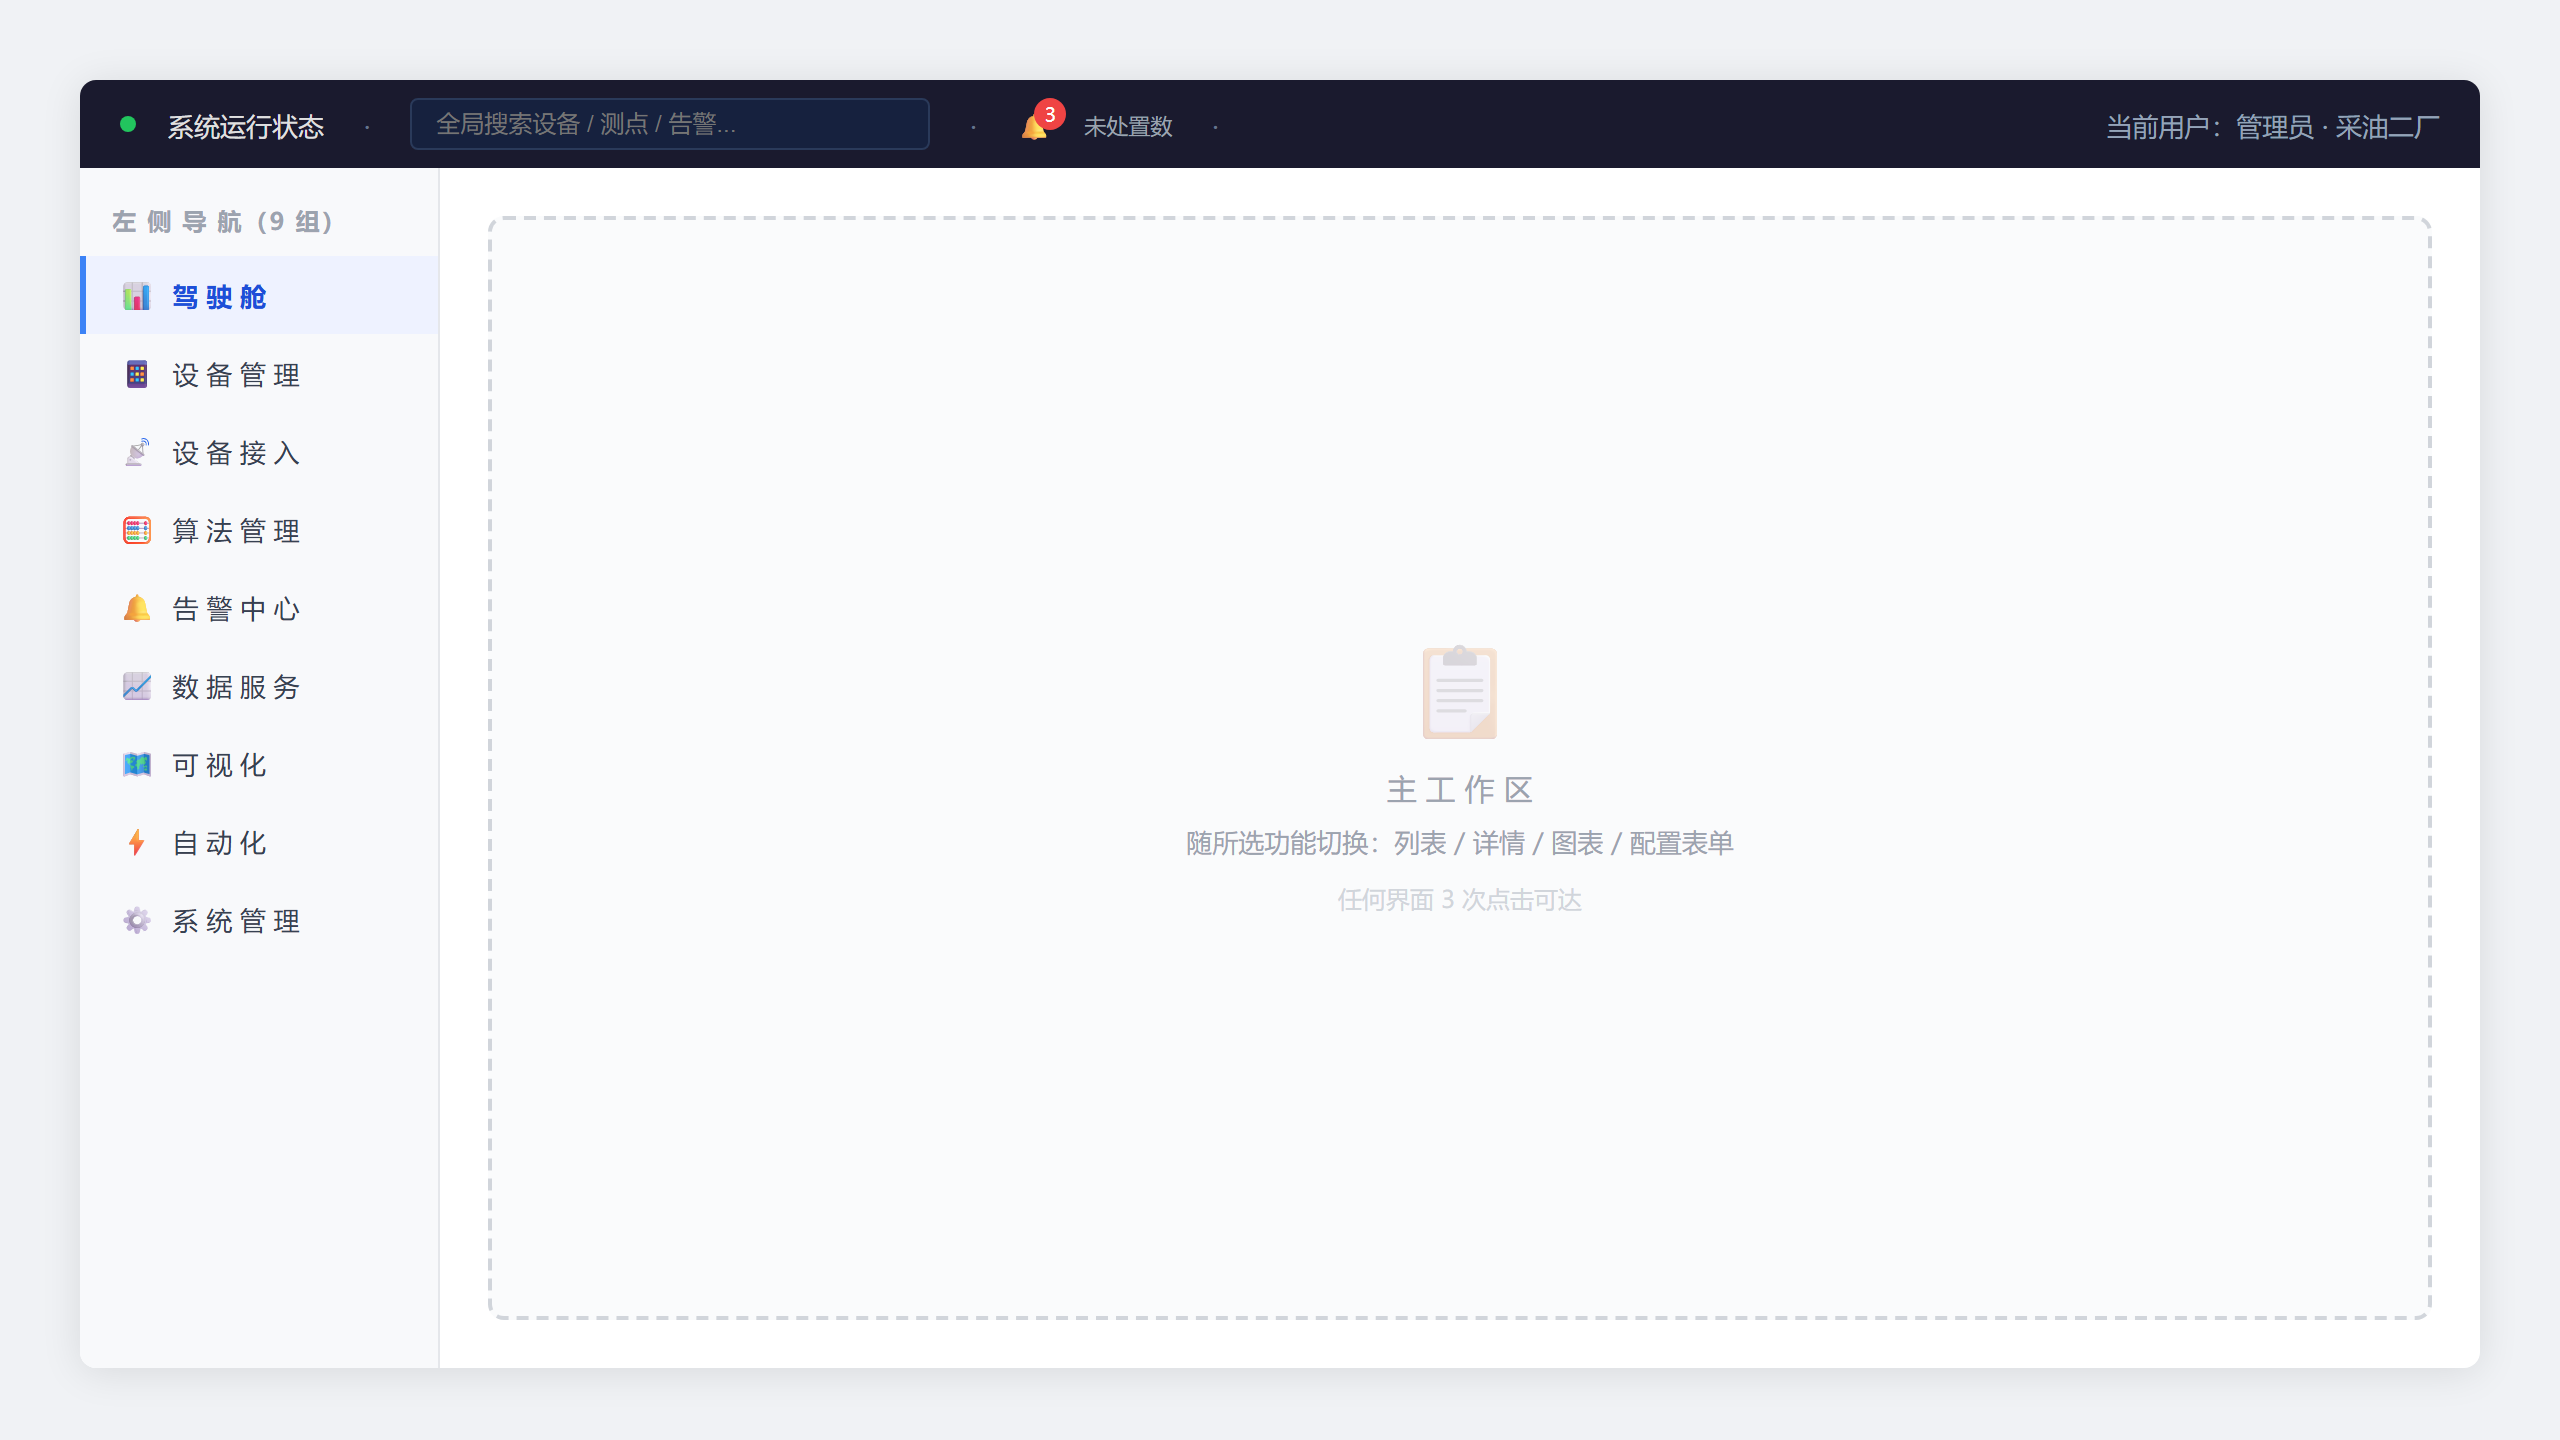
\includegraphics[width=0.96\textwidth]{管理后台布局图.png}
\caption{管理后台总体布局——9 组导航对应 IoT 平台标准模块，任何界面 3 次点击可达}
\end{figure}

\subsection{八张关键界面蓝图}

以下八张界面覆盖领导与运维\textbf{90\% 以上的日常使用场景}，每张界面附"领导视角一句话"——这个界面回答什么问题。

\begin{table}[H]\centering
\caption{界面蓝图清单（每张界面回答一个领导关心的问题）}
\begin{tabular}{p{2.6cm} p{6.8cm} p{4.4cm}}
\toprule
\textbf{界面} & \textbf{核心内容（后台支撑服务往这里放）} & \textbf{领导视角一句话} \\
\midrule
\textbf{① 驾驶舱}（大屏看板） & 链路健康率/采集完整率/设备在线率 KPI 卡片墙；C 位全油田采集链路拓扑图（状态着色）；告警滚动列表（红色高亮）；KPI/告警秒级刷新 & "一眼看全油田：一切正常吗？" \\
\textbf{② 设备管理} & 设备台账、五态状态（在线/离线/未激活/异常/冻结）+ 判离线规则、设备详情六页签（台账/实时/历史/告警/趋势/采集日志）、物模型自动配点（G1--G8 油水井 64 点）、A11 既有点位原样映射 & "资产管得住，配点不用手工" \\
\textbf{③ 设备接入} & 静态/动态终端分视图、链路状态码+语义色（正常/降频/离线/告警）、实时采集频率、\textbf{断网补传进度条}、网关在线地图；双路采集（静态客户端/动态桥接）、10 家网关厂家适配入口 & "每台设备都接上来了吗？" \\
\textbf{④ 算法管理} & 15 种内置算法库、作业区定制算法注册制、算法覆盖率/命中率指标、算法启停/版本/A--B 对比/逐井调优、可视化规则编排 & "定制算法注册了几个、算得准不准？" \\
\textbf{⑤ 告警中心} & 四级告警（Critical/Error/Warning/Info）、确认/清除双动作（未确认未清除计数）、分级通知升级链（超时逐级升级、确认即停）、\textbf{工单流转闭环}（发现→确认→处置→归档） & "异常有人管、处置可追溯" \\
\textbf{⑥ 数据服务} & 多粒度统计（日/月/年）、时间轴拖拽回放、健康日报自动生成、横向对比；\textbf{REST API 数据接口}、TDengine 时序查询、PostgreSQL 关系查询 & "趋势看得到，数据取得出" \\
\textbf{⑦ 可视化} & 作业区→设备→链路全拓扑（兼作驾驶舱 C 位主视觉）；\textbf{拖拽式仪表盘组态}（图表/指标卡/趋势图）；GIS 地图层级下钻；点击任一节点下钻详情 & "整个油田的采集结构一图了然" \\
\textbf{⑧ 自动化} & \textbf{规则引擎联动}：采集触发→条件判定→动作执行（自动调频/降级/重启）；\textbf{场景编排}：批量设备配置下发、定时巡检任务、断网自动补传触发 & "能不能自己跑、少让人盯着？" \\
\textbf{⑨ 系统管理} & 用户/角色/权限（角色化界面裁剪：领导/调度/运维千人千面，大屏+PC+移动三端）、审计日志（操作全留痕）、国密 SM2/3/4 安全配置、信创全栈适配 & "谁能看什么、谁动过什么，都有数" \\
\bottomrule
\end{tabular}
\end{table}

\subsection{数据驾驶舱大屏效果示意}

\begin{figure}[H]\centering
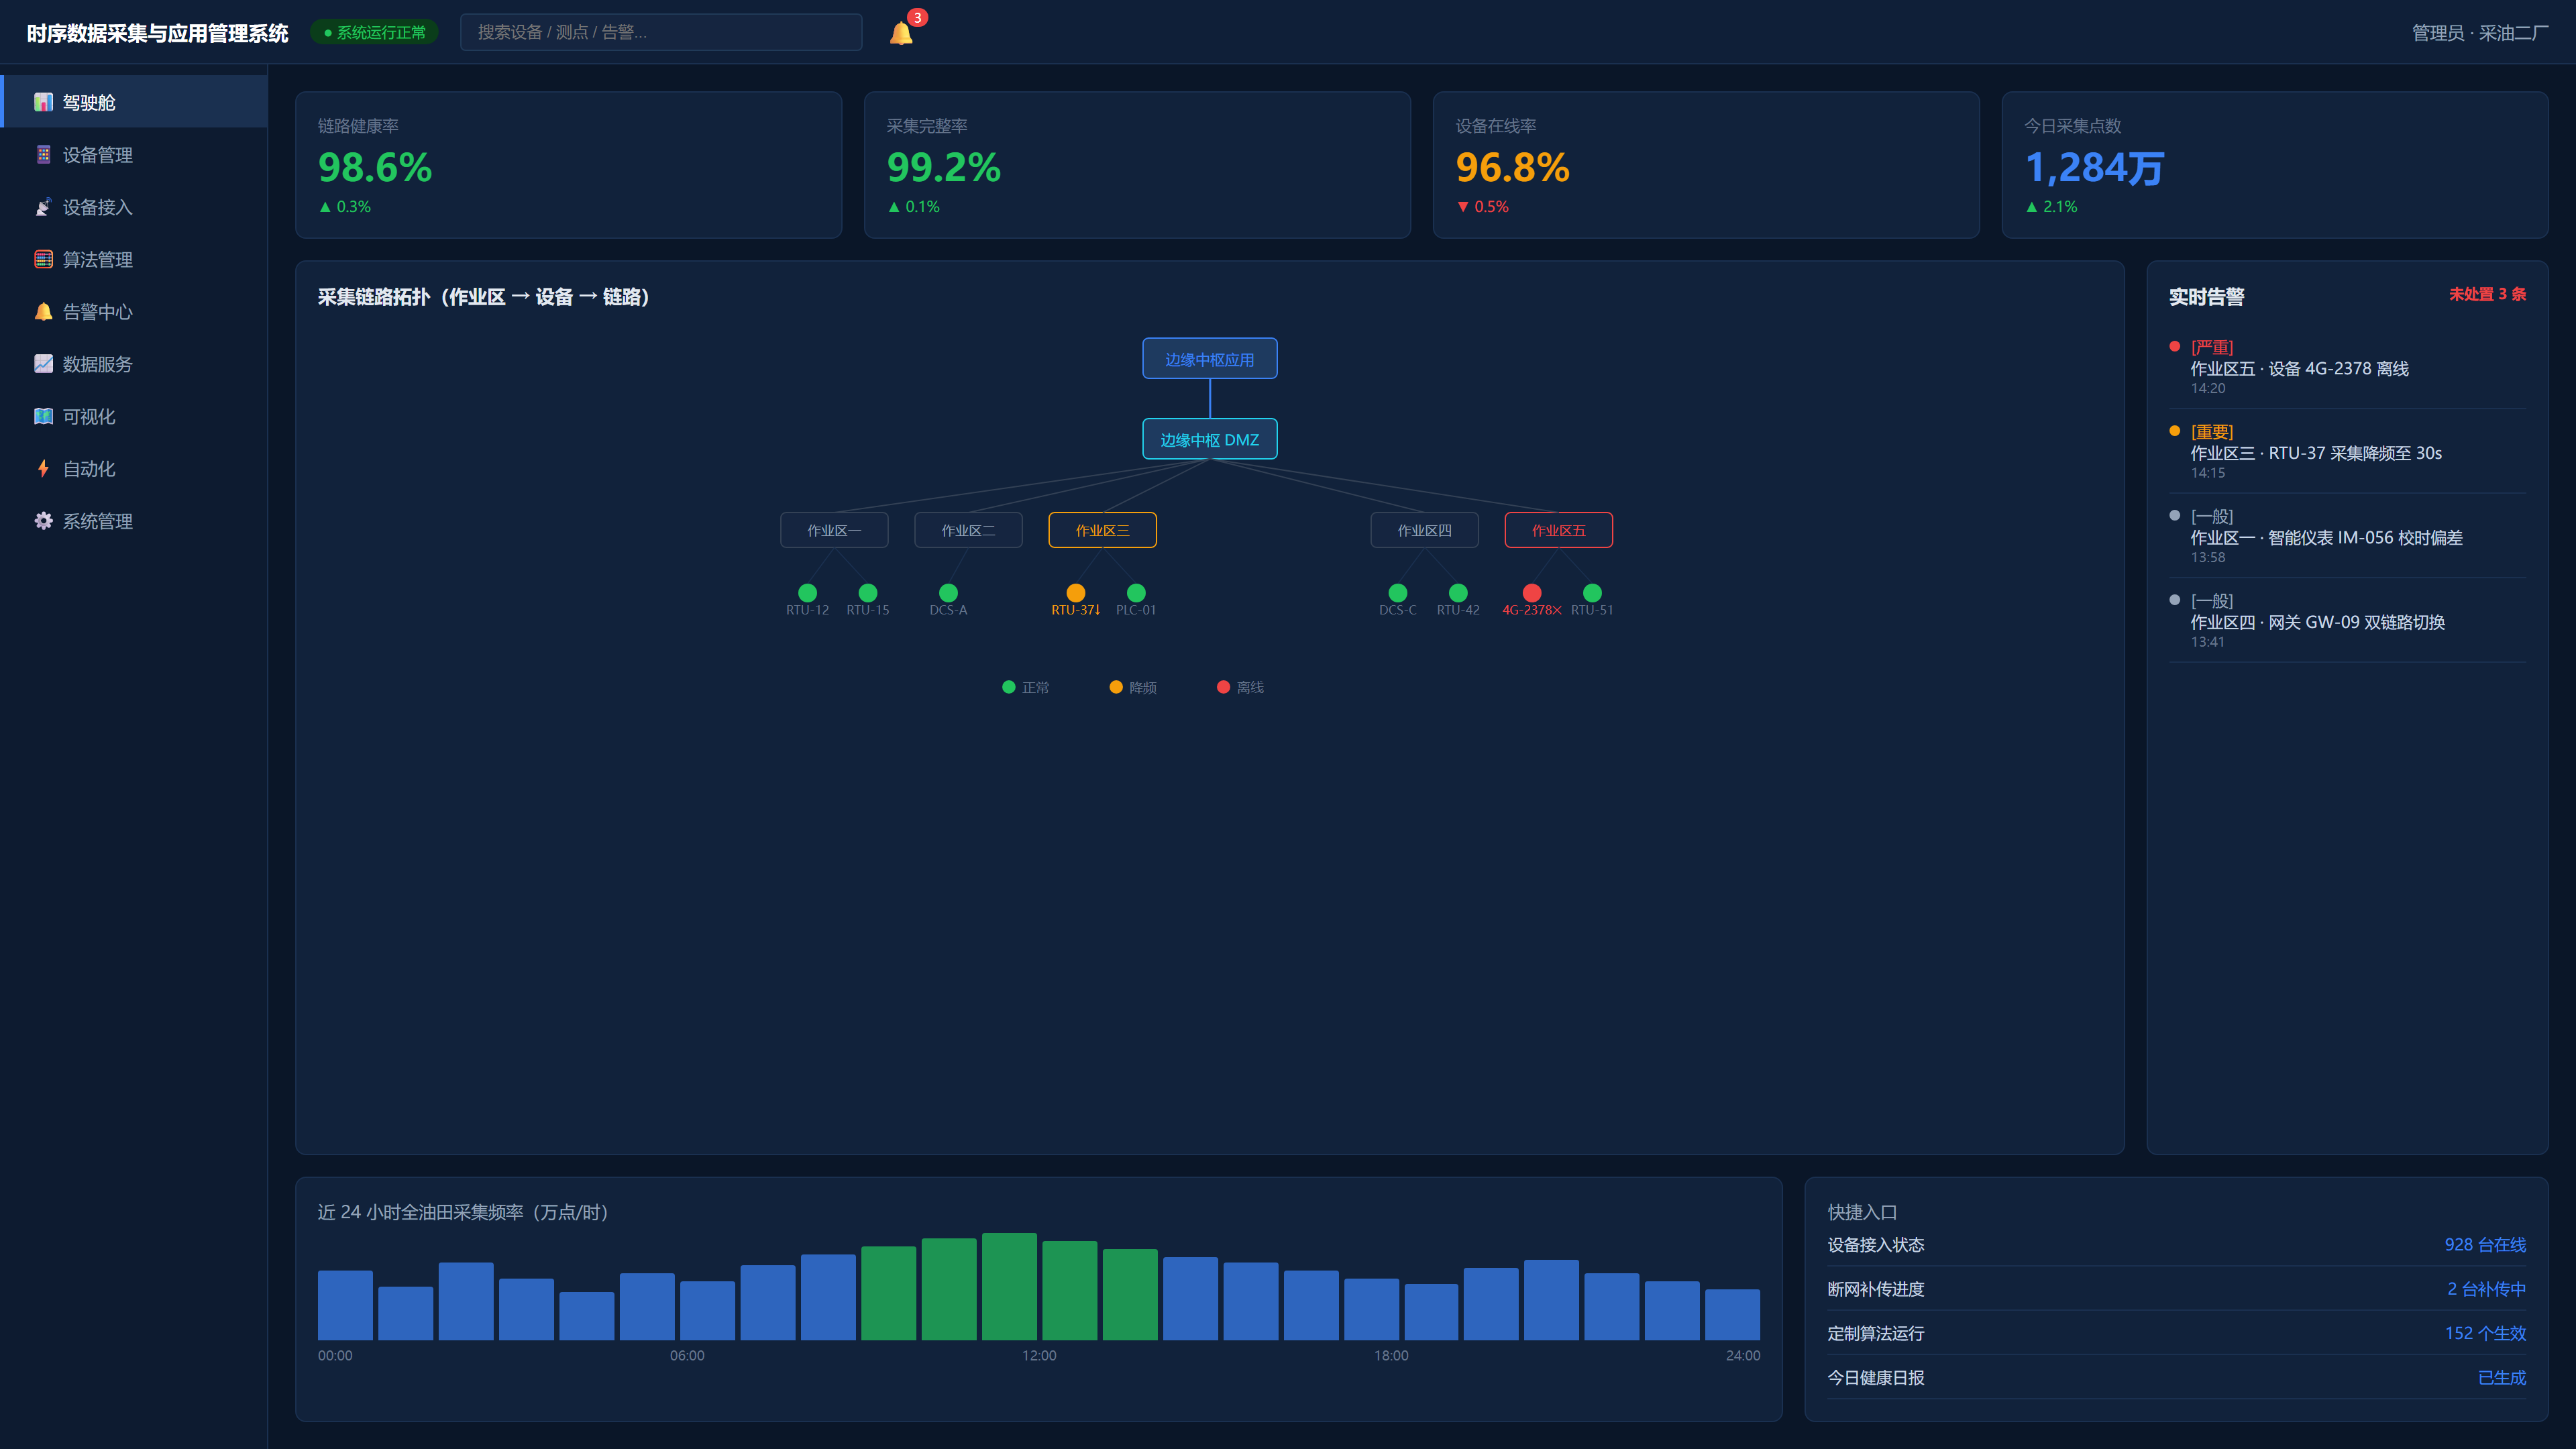
\includegraphics[width=0.94\textwidth]{驾驶舱大屏截图.png}
\caption{数据驾驶舱大屏效果示意——C 位采集链路拓扑（状态着色）、左侧结果性指标卡片、右侧告警滚动列表、底部采集频率趋势（界面效果示意，非实际运行数据）}
\end{figure}

\subsection{四张核心界面示意}

\begin{figure}[H]\centering
\begin{tikzpicture}[
  font=\scriptsize,
  box/.style={draw, rounded corners=2pt, align=left, text width=7.2cm, inner sep=4pt},
  hdr/.style={font=\footnotesize\bfseries, fill=gray!10}
]
% 左列
\node[box] (s1) {{\bfseries ① 驾驶舱（大屏，领导首屏）}\\[2pt]
\textbullet{} C 位主视觉：全油田采集链路拓扑图（状态着色）\\
\textbullet{} 大数字卡片（结果口径）：链路健康率 \textbullet{} 采集完整率 \textbullet{} 设备在线率\\
\textbullet{} 右侧告警滚动列表：未处置数红色高亮，逐条下钻\\
\textbullet{} 实时曲线：全油田采集频率分布\\
\emph{领导视角：全油田 10 秒看懂} };
\node[box, below=0.6cm of s1] (s2) {{\bfseries ② 设备接入（数据怎么上来）}\\[2pt]
\textbullet{} 终端类型筛选：静态 IP / 动态 IP / 移动网关\\
\textbullet{} 每台设备：链路状态 · 频率档位 · 最近数据时间\\
\textbullet{} 断网缓存：离线台数 · 补传进度条 · 时序对齐校验\\
\textbullet{} 双路采集入口：静态采集/动态桥接 · 10 家网关厂家适配\\
\emph{领导视角：链路是否健康、有没有漏采} };
% 右列
\node[box, right=0.8cm of s1] (s3) {{\bfseries ③ 算法管理（流式计算）}\\[2pt]
\textbullet{} 内置算法库：15 种（工况诊断/预警/统计类）开箱即用\\
\textbullet{} 定制算法注册区：每作业区 $\geq$1 个，注册制、批量校验\\
\textbullet{} 逐井调优：单井参数调整、A/B 对比、版本回滚\\
\textbullet{} 可视化规则编排：拖拽式配置触发条件与动作\\
\emph{领导视角：定制算法价值直接可见} };
\node[box, below=0.6cm of s3] (s4) {{\bfseries ④ 告警中心（闭环处置）}\\[2pt]
\textbullet{} 四级告警分级列表（Critical 置顶红标）\\
\textbullet{} 确认/清除双动作：未确认未清除计数常驻可见\\
\textbullet{} 升级链：超时未确认逐级升级（声光/短信/平台），确认即停\\
\textbullet{} 工单流转：发现 $\rightarrow$ 确认 $\rightarrow$ 处置 $\rightarrow$ 归档\\
\emph{领导视角：异常有人管、处置可追溯} };
\end{tikzpicture}
\caption{四张核心界面示意——驾驶舱、设备接入、算法管理、告警中心}
\end{figure}

\subsection{其余界面示意}

\begin{figure}[H]\centering
\begin{tikzpicture}[
  font=\scriptsize,
  box/.style={draw, rounded corners=2pt, align=left, text width=7.2cm, inner sep=4pt},
  hdr/.style={font=\footnotesize\bfseries, fill=gray!10}
]
\node[box] (s1) {{\bfseries ⑤ 设备管理（台账与物模型）}\\[2pt]
\textbullet{} 设备台账：全油田设备清单（厂家/型号/协议/链路）\\
\textbullet{} 设备状态五态：在线/离线/未激活/异常/冻结（判离线规则明确）\\
\textbullet{} 设备详情六页签：台账/实时/历史/告警/趋势/采集日志\\
\textbullet{} 物模型自动配点：G1--G8 油水井一键配点生成 64 点\\
\emph{领导视角：资产管得住，配点不用手工} };
\node[box, below=0.5cm of s1] (s2) {{\bfseries ⑥ 数据服务（报表与数据接口）}\\[2pt]
\textbullet{} 多粒度统计：日/月/年聚合、作业区横向对比\\
\textbullet{} 历史回放：时间轴拖拽定位任意时段曲线\\
\textbullet{} 健康日报：在线率/完整率/成功率自动生成\\
\textbullet{} REST API：时序/关系数据标准化接口对外提供\\
\emph{领导视角：趋势看得到，数据取得出} };
\node[box, right=0.8cm of s1] (s3) {{\bfseries ⑦ 可视化（拓扑与仪表盘）}\\[2pt]
\textbullet{} 采集链路拓扑：作业区$\rightarrow$设备$\rightarrow$链路逐级展开\\
\textbullet{} 状态着色：正常/降频/离线/告警，点击下钻\\
\textbullet{} 拖拽式仪表盘：图表/指标卡/趋势图自由组态\\
\textbullet{} GIS 地图：油田$\rightarrow$作业区$\rightarrow$站库层级下钻\\
\emph{领导视角：一图看全、想怎么看自己搭} };
\node[box, below=0.5cm of s3] (s4) {{\bfseries ⑧ 自动化（规则联动与场景编排）}\\[2pt]
\textbullet{} 规则引擎：采集触发 $\rightarrow$ 条件判定 $\rightarrow$ 动作执行\\
\textbullet{} 场景编排：批量设备配置下发、定时巡检任务\\
\textbullet{} 联动动作：自动调频/降级/重启、断网自动补传触发\\
\textbullet{} 设备影子（Shadow）：上报值 vs 期望值，状态同步\\
\emph{领导视角：能不能自己跑、少让人盯着} };
\node[box, below=0.2cm of s4, fill=yellow!5, minimum height=1.5cm] (s5) {{\bfseries ⑨ 系统管理（角色与安全）}\\[2pt]
\textbullet{} 角色化界面裁剪：领导/调度/运维千人千面，大屏+PC+移动三端\\
\textbullet{} 审计日志：操作全留痕、可追溯 · 国密 SM2/3/4 加密 · 信创全栈适配\\
\emph{领导视角：谁看什么、谁动过什么都有记录} };
\end{tikzpicture}
\caption{其余五张界面示意——设备管理、数据服务、可视化、自动化、系统管理}
\end{figure}

\subsection{三个界面亮点（对标行业主流平台界面惯例）}

\begin{itemize}[leftmargin=*]
  \item \textbf{断网补传进度可视化}：断网设备的数据补传进度（离线台数、补传进度条、时序对齐校验）实时可见——\textbf{链路断过，领导也能看出"数据补回来了"}。多数平台仅有"断网告警"、缺少"补传进度"界面，这是本系统的少见亮点；
  \item \textbf{采集链路拓扑作 C 位主视觉}：驾驶舱中央以"作业区 $\rightarrow$ 设备 $\rightarrow$ 链路"拓扑图承担主视觉（对标行业大屏"一张图"惯例），状态着色，一处异常一眼可辨；
  \item \textbf{结果性指标口径}：首屏 KPI 以"链路健康率、采集完整率"等结果口径呈现（对标行业"在线率"头号指标惯例），让领导先看到\textbf{业务结果}，而非过程数据罗列。
\end{itemize}

% ═══════════════════════════════════════════
\section{界面与底座的贯通：一次点击背后的数据流}

每张界面都不是孤立的——\textbf{界面是五层架构的"窗口"，背后是底座服务在实时工作}：

\begin{longtable}{p{2.4cm} p{5.4cm} p{6.0cm}}
\toprule
\textbf{界面} & \textbf{看到的} & \textbf{背后的底座服务} \\
\midrule
\endfirsthead
\multicolumn{3}{c}{(续表)} \\
\toprule
\textbf{界面} & \textbf{看到的} & \textbf{背后的底座服务} \\
\midrule
\endhead
驾驶舱 & 链路健康率/采集完整率/告警滚动 & 采集引擎实时统计 + 告警引擎汇总 + 消息中间件推送（秒级） \\
设备管理 & 台账/点位/配点状态/五态生命周期 & 物模型匹配服务 + 主数据体系 + 设备动态感知 \\
设备接入 & 链路状态/频率档位/补传进度/网关地图 & 双路采集（静态客户端/动态桥接）+ 动态调频调度 + 断网缓存补传 \\
算法管理 & 算法库/定制注册/逐井调优/规则编排 & 流式计算引擎（15 内置 + 定制注册制）+ 可视化规则编排 \\
告警中心 & 告警分级/工单流转/通知记录/升级链 & 流式告警规则引擎 + 四级告警闭环 + 差异化通知 + 工单服务 \\
数据服务 & 聚合统计/回放/健康日报/数据 API & 历史计算模块 + 多粒度聚合 + 报告自动生成 + REST API 网关 \\
可视化 & 拓扑/仪表盘组态/GIS 下钻 & 设备动态感知 + 链路健康台账 + 拖拽式仪表盘引擎 \\
自动化 & 规则联动/场景编排/批量下发 & 规则引擎 + 场景调度器 + 设备影子（Shadow） \\
系统管理 & 权限/审计/角色裁剪/安全配置 & 用户权限服务 + 全链路审计追溯 + 国密安全组件 + 信创适配层 \\
\bottomrule
\end{longtable}

\subsection{功能归属：边缘代理 vs 边缘中枢}

\noindent
\textbf{边缘代理}——部署在作业区 IO 服务器上（生产网），负责\textbf{把数据采上来}：
\begin{itemize}[leftmargin=*]
  \item 协议解析（A11/Modbus/OPC DA/IEC104）· 双路采集（静态客户端/动态桥接）· 设备动态感知
  \item 本地缓存 + 断网补传 · 动态调频 · 物模型自动配点
  \item 对应报价板块三（边缘采集）· 板块四（作业区定制）· 运行在 IO 服务器上
\end{itemize}

\noindent
\textbf{边缘中枢}——部署在 DMZ 区（麒麟 Linux），负责\textbf{把数据汇起来、算出来、呈现出来}：
\begin{itemize}[leftmargin=*]
  \item MQTT 千万级汇聚 · 流式计算引擎 · 告警规则引擎 · 混合存储
  \item 驾驶舱大屏 · 管理后台 9 界面 · REST API · 可视化仪表盘
  \item 对应报价板块一（软件产品）· 板块二（汇聚对接）· 运行在 DMZ/办公网
\end{itemize}

\subsection{底座服务到界面模块的映射（后台往哪放）}

每个界面模块背后是对应的服务组件，\textbf{不是空壳页面——每个菜单点进去都有代码在跑}：

\begin{table}[H]\centering
\caption{9 大界面模块 × 底座服务 × 前端 View 三层对应}
{\small
\begin{tabular}{p{1.8cm} p{4.3cm} p{3.8cm} p{3.2cm}}
\toprule
\textbf{界面模块} & \textbf{背后底座服务} & \textbf{运行位置} & \textbf{前端 View（已实现）} \\
\midrule
\textbf{驾驶舱} & collector.py + alarm\_engine.py + dashboard\_edge\_api.py & 边缘中枢 & DashboardView · SystemOverview \\
\textbf{设备管理} & device.py + thing\_model.py + asset\_api.py + parse\_lite.py & 边缘中枢 & DeviceListView · DeviceDetailView · ProductsView · ChannelView \\
\textbf{设备接入} & protocols/ 11 协议 + collector.py + gateway\_dynamic.py + modbus\_auto\_identify.py & \textbf{边缘代理} & EdgeProxyView · IOCloneView · SimulatorView · MqttToolView \\
\textbf{算法管理} & stream\_engine.py + flow\_learner.py + rules\_engine.py + phm\_engine.py & 边缘中枢 & StreamView · PhmView \\
\textbf{告警中心} & alarm\_engine.py + safety\_rules.py + push\_engine.py & 边缘中枢 & AlarmListView \\
\textbf{数据服务} & tdengine.py + postgres.py + oracle\_bridge.py + report\_generator.py & 边缘中枢 & ReportsView · TelemetryView · AmisTestView \\
\textbf{可视化} & admin\_panel.py + dashboard\_edge\_api.py + dgiot\_schema.py & 边缘中枢 & TopologyView · HmiView · ScadaView \\
\textbf{自动化} & rules\_engine.py + shadow.py + push\_engine.py + zone\_adapter.py & \textbf{边缘代理} & FdeWizardView · MaintenanceView \\
\textbf{系统管理} & auth.py + sm\_crypto.py + system\_api.py + tenant\_api.py & 边缘中枢 & UsersView · LoginView · GraphRagView \\
\bottomrule
\end{tabular}
}
\end{table}

{\footnotesize 前端 View 路径：\texttt{D:\textbackslash ai\textbackslash dgiot\_lite\textbackslash frontend-vue\textbackslash src\textbackslash views/}（25 个 View 全部对应到 9 模块，无遗漏）}

\textbf{界面-底座贯通的意义}：领导在驾驶舱看到的每一个数字，都是\textbf{采集层、存储层、计算层实时协作的结果}——这也是本系统与"只有报表没有采集"的信息系统的本质区别：\textbf{数据是自己采的、自己算的、自己管的，不是从别的系统倒过来的}。

% ═══════════════════════════════════════════
\section{分期开放节奏}

界面随工程三阶段渐进接入逐步开放，\textbf{每一步都有东西可看、可验证}：

\begin{table}[H]\centering
\caption{三阶段界面开放节奏（对应三阶段渐进接入）}
\begin{tabular}{p{2.2cm} p{5.6cm} p{6.0cm}}
\toprule
\textbf{阶段} & \textbf{采集侧进展} & \textbf{界面侧可看内容} \\
\midrule
\textbf{阶段一：观察} & 静态 IP 终端客户端主动采集上线 & 设备管理、设备接入（静态视图）、驾驶舱雏形（首批作业区数据） \\
\textbf{阶段二：桥接复制} & 动态 IP 终端抢占原地址端口桥接（复制 + 原样转发，原 A11 业务不断） & 设备接入（动态视图）、断网补传进度、可视化接入 \\
\textbf{阶段三：稳定并行} & 全作业区覆盖、调频策略逐区生效 & 算法管理（定制算法注册）、告警中心闭环、数据服务、驾驶舱全量 \\
\bottomrule
\end{tabular}
\end{table}

\textbf{试点安排}：试点 10 作业区先行验证（功能完整落地），再按实际覆盖范围扩展二期——\textbf{每进入一个作业区，领导在该区就能看到完整的"采-算-告-看"闭环}。

% ═══════════════════════════════════════════
\section{附录：界面功能单独核算（另行报价）}

{\small\bfseries\color{red!70!black} 声明：本附录所列界面功能不在报价书总价（725.04 万元）内，另行核算、另行报价。报价书各板块已含物模型、数据服务与接口配合基础，本附录仅核算界面呈现层，避免重复计价。}

\subsection{界面功能清单}

\begin{table}[H]\centering
\caption{界面功能清单（10 项 · 全部自研 · 源码交付 · 另行报价参考）}
\begin{tabular}{p{3.2cm} p{5.8cm} p{2.0cm} p{1.8cm}}
\toprule
\textbf{界面功能} & \textbf{功能说明} & \textbf{工作类型} & \textbf{参考核算（万元）} \\
\midrule
综合监控大盘 & 设备运行状态总览、采集通道健康度、告警分布态势、公式计算实时状态 & 自研 & 15.0 \\
资产全生命周期管理 & A2/A5 资产树（油田$\rightarrow$作业区$\rightarrow$站库$\rightarrow$井组$\rightarrow$单设备五级）、注册/监测/维护/退役全周期 & 自研 & 15.0 \\
GIS 地图下钻 & 油田$\rightarrow$作业区$\rightarrow$站库$\rightarrow$井组地图层级下钻、设备点位标注与状态着色 & 自研 & 8.0 \\
联动钻取分析 & 告警卡片$\rightarrow$设备详情$\rightarrow$原始时序数据一键下钻、采集-计算-存储全链路追溯 & 自研 & 8.0 \\
报表中心 & 日/周/月报自动生成与推送、HTML/JSON 导出 & 自研 & 10.0 \\
告警处置工作台 & 四级告警闭环看板、电话/短信/APP 通知记录 & 自研 & 10.0 \\
配置管理界面 & 采集频次/告警阈值/数据保留策略集中配置、物模型与点表配置、规则编排 & 自研 & 12.0 \\
运维管控界面 & 设备/日志/任务/系统健康自监控、分布式节点状态、网关台账与体检报告 & 自研 & 10.0 \\
拖拽式仪表盘 & 个性化仪表盘组态（拖拽图表/指标卡/趋势图）、模板保存与版本管理 & 自研 & 8.0 \\
数据湖门户嵌入 & 管理界面嵌入数据湖门户、单点登录与菜单集成联调 & 自研 & 8.0 \\
\midrule
\textbf{合计} & \textbf{10 项} & \textbf{全部自研、源码交付} & \textbf{104.0（另行报价）} \\
\bottomrule
\end{tabular}
\end{table}

\subsection{与报价书的关系}

\begin{itemize}[leftmargin=*]
  \item 报价书总价 725.04 万元 \textbf{不含}本表 104 万元；界面功能以补充协议方式另行确认后执行。
  \item 本表界面功能所依赖的数据服务（物模型、点位数据、接口）已含于报价书板块一/三/四，此处仅核算呈现层，不存在重复计价。
  \item 界面功能的验收标准与报价书一致（500 万测点 3s 查询、5 万并发下页面可用性），随联调测试一并验证。
\end{itemize}

\vspace{1em}
\noindent\hrulefill

\begin{center}
\small 编制单位：迪格(杭州)物联科技有限公司 \quad 2026-08 \quad 配套：报价书、报价表 V10、附件②③④⑥、全景论证、附图（系统功能树与网络拓扑）
\end{center}

\end{document}
